% =============================================================================
\section{Comparison with an exact method}
\label{sec:wigner-bec:mm}
% =============================================================================

It is usually problematic to perform a comparison with an exact method for the functional truncated Wigner, since it is applied to the systems with many modes and many particles, for which no exact methods exist.
It is possible though to do this for the multimode truncated Wigner with only a few modes.
Such systems are well within the area of applicability for first-principle exact methods such as number state expansions.

In the paper~\cite{Opanchuk2012a} we considered a two-well four-mode \abbrev{bec} system with the Hamiltonian
\begin{eqn}
    \hat{H}
    = \frac{1}{2} \sum_{i,j=1}^2 \tilde{g}_{ij} \left(
        \hat{a}_i^\dagger \hat{a}_j^\dagger \hat{a}_j \hat{a}_i
        + \hat{b}_i^\dagger \hat{b}_j^\dagger \hat{b}_j \hat{b}_i
        \right).
\end{eqn}
In this section we are only interested in a simple local case with no interaction between wells, so we can simplify the Hamiltonian to
\begin{eqn}
    \hat{H}
    = \frac{1}{2} \sum_{i,j=1}^2 \tilde{g}_{ij}
        \hat{a}_i^\dagger \hat{a}_j^\dagger \hat{a}_j \hat{a}_i.
\end{eqn}
The evolutions starts from the coherent state
\begin{eqn}
\label{eqn:wigner-bec:mm:initial-cond}
    \Psi(0)
    =
        \ket{\sqrt{N_a / 2}}_{a_1}
        \ket{\sqrt{N_a / 2}}_{a_2},
\end{eqn}
where $N_a$ stands for the initial total number of atoms in the first and the second well respectively.
The evolution of the system is governed by the master equation
\begin{eqn}
\label{eqn:wigner-bec:mm:master-eqn}
    \frac{\upd \hat{\rho}}{\upd \tau}
    = -i \left[ \hat{H}, \hat{\rho} \right].
\end{eqn}
After the transformation to the \abbrev{fpe} form with \thmref{mm-wigner:mm:correspondences}, truncation, and further transformation with \thmref{fpe-sde:corr:mc-fpe-sde}, this results in the equivalent system of \abbrev{sde}s
\begin{eqn}
    \upd \begin{pmatrix}
        \alpha_1 \\ \alpha_2
    \end{pmatrix}
    = -i \begin{pmatrix}
        \alpha_1 (\tilde{g}_{11} |\alpha_1|^2 + \tilde{g}_{12} |\alpha_2|^2) \\
        \alpha_2 (\tilde{g}_{22} |\alpha_2|^2 + \tilde{g}_{12} |\alpha_1|^2)
    \end{pmatrix} \upd \tau.
\end{eqn}
These equations can be solved numerically, which in our case was done with XMDS (see \appref{numerical} for details), and the operator moments given by \thmref{mm-wigner:mm:moments} can be used to obtain required observables.

On the other hand, the master equation~\eqnref{wigner-bec:mm:master-eqn} can be solved exactly using a number state expansion~\cite{Opanchuk2012a}.
% acknowledgement
The theoretical derivations and the results of the numerical calculations for this method were provided by Q.-Y.~He.
In the Heisenberg representation the equations of motion for the first well (with the absence of coupling of any kind, the evolution in the wells is independent) are
\begin{eqn}
    \frac{\upd \hat{a}_i}{\upd t}
    = i \left[ \hat{H}, \hat{a}_i \right]
    = -i \sum_{j=1}^2 g_{ij} \hat{N}_j \hat{a}_i,
\end{eqn}
and their solution is
\begin{eqn}
\label{eqn:wigner-bec:mm:exact-a}
    \hat{a}_i(\tau)
    = \exp \left( -i \sum_{j=1}^2 g_{ij} \hat{N_j} \tau \right).
\end{eqn}
The initial conditions~\eqnref{wigner-bec:mm:initial-cond} can be, in turn, expanded as
\begin{eqn}
    \Psi_a(0)
    =
        \sum_{m=0}^{\infty} C_m^{(1)} \ket{m}_{a_1}
        \sum_{n=0}^{\infty} C_n^{(2)} \ket{n}_{a_2},
\end{eqn}
and used to calculate any required moments $f(\hat{a}_1^\dagger, \hat{a}_1, \hat{a}_2^\dagger, \hat{a}_2)$ at time $\tau$ as
\begin{eqn}
\label{eqn:wigner-bec:mm:exact-f}
    \langle f(\hat{a}_1^\dagger, \hat{a}_1, \hat{a}_2^\dagger, \hat{a}_2) \rangle
    ={} &
        \sum_{k,l,m,n=0}^{\infty} C_k^{(1)} C_l^{(2)} C_m^{(1)} C_n^{(2)} \\
    & \quad \times \bra{k}_{a_1} \bra{l}_{a_2}
        f(\hat{a}_1^\dagger(\tau), \hat{a}_1(\tau), \hat{a}_2^\dagger(\tau), \hat{a}_2(\tau))
        \ket{m}_{a_1} \ket{n}_{a_2}.
\end{eqn}

For the comparison we will take several quantities that were calculated for the system in question~\cite{Opanchuk2012a}.
We will not go into detail about their physical meaning here, as they is not the primary focus of this thesis.
First we introduce phase-rotated Schwinger spin operator measurements for each well as
\begin{eqn}
    \hat{J}_A^X
    & = \frac{1}{2} \left(
            \hat{a}_{2}^{\dagger} \hat{a}_{1} e^{i\Delta\theta}
            +\hat{a}_{1}^{\dagger} \hat{a}_{2} e^{-i\Delta\theta}
        \right),\\
    \hat{J}_A^Y & = \frac{1}{2i} \left(
            \hat{a}_{2}^{\dagger} \hat{a}_{1} e^{i\Delta\theta}
            - \hat{a}_{1}^{\dagger} \hat{a}_{2} e^{-i\Delta\theta}
        \right),\\
    \hat{J}_A^Z & = \frac{1}{2} \left(
        \hat{a}_{2}^{\dagger} \hat{a}_{2}
        - \hat{a}_{1}^{\dagger} \hat{a}_{1}\right),
\end{eqn}
where $\Delta\theta = \pi / 2 - \arg \langle \hat{a}_2^\dagger \hat{a}_1 \rangle$ is the phase difference between the two modes in a well.

We consider all possible orthogonal pairs of spin operators $\hat{J}^\theta$, $\hat{J}^{\theta+\pi/2}$ in the plane orthogonal to $\hat{J}_Y^A$, where $\hat{J}^\theta$ is defined as
\begin{eqn}
    \hat{J}^\theta
    =   \hat{J}^{Z} \cos \theta
        + \hat{J}^{X} \sin \theta.
\end{eqn}
These pairs obey the Heisenberg uncertainty relation
\begin{eqn}
    \Delta\hat{J}^{\theta} \Delta\hat{J}^{\theta+\pi/2}
    \geq
    |\langle\hat{J}^{Y}\rangle|/2.
\end{eqn}
Even with this limit on the pair, the variance of one of the spins in the pair can be reduced below the Heisenberg limit:
\begin{eqn}
    \Delta^{2}\hat{J}^{\theta} < |\langle\hat{J}^{Y}\rangle|/2,
\end{eqn}
which is referred to as the ``spin squeezed state''.

It can be shown~\cite{Opanchuk2012a} that the optimal squeezing angle is
\begin{eqn}
    \theta
    = \frac{1}{2} \arctan \left(
        \frac{2\langle\hat{J}_{A}^{Z},\hat{J}_{A}^{X}\rangle}{%
            \Delta^{2}\hat{J}_{A}^{Z} - \Delta^{2}\hat{J}_{A}^{X}}
    \right),
\end{eqn}
and the degree of squeezing can be quantified as
\begin{eqn}
\label{eqn:wigner-bec:mm:squeezing}
    S^{\theta,\theta+\pi/2}
    = \frac{\Delta^{2}\hat{J}_{A}^{\theta,\theta+\pi/2}}{%
        \vert\langle\hat{J}_{A}^{Y}\rangle\vert/2}.
\end{eqn}
Here we denoted the pair correlation
\begin{eqn}
    \langle\hat{J}_{A}^{Z},\hat{J}_{A}^{X}\rangle
    = \frac{1}{2} \left(
            \langle\hat{J}_{A}^{Z}\hat{J}_{A}^{X}\rangle
            + \langle\hat{J}_{A}^{X}\hat{J}_{A}^{Z}\rangle
            - 2\langle\hat{J}_{A}^{Z}\rangle\langle\hat{J}_{A}^{X}\rangle
        \right).
\end{eqn}

\begin{figure}
    \centerline{%
    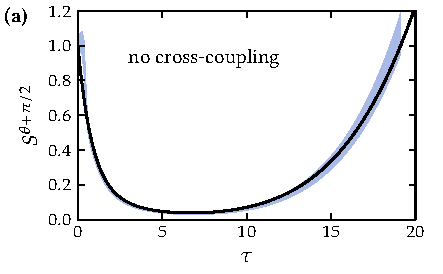
\includegraphics{figures_generated/exact/squeezing_nocc_100.pdf}%
    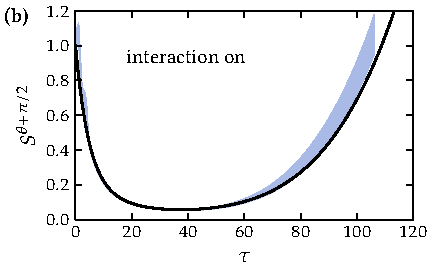
\includegraphics{figures_generated/exact/squeezing_cc_100.pdf}}

    \caption[Comparison of Wigner simulated local squeezing with an exact method]{
    Comparison of the Wigner simulated time-dependent local squeezing (blue bands; the width corresponds to the estimated sampling error) against the exact results (black lines).
    Trajectories used: $2,000$.
    The plots correspond to \textbf{(a)} the case of no inter-component interaction ($\tilde{g}_{12} = 0$, $\tilde{g}_{11} = \tilde{g}_{22} = 1 / N_A$), and \textbf{(b)} strong inter-component interaction ($\tilde{g}_{ij} = a_{ij} / (a_{11} N_A)$, where $a_{11} = 100.4$, $a_{12} = 80.8$ and $a_{22} = 95.5$).}%endcaption

    \label{fig:wigner-bec:mm:squeezing-comparison}
\end{figure}

\begin{figure}
    \centerline{%
    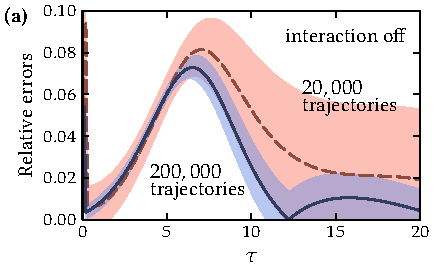
\includegraphics{figures_generated/exact/squeezing_nocc_err.pdf}%
    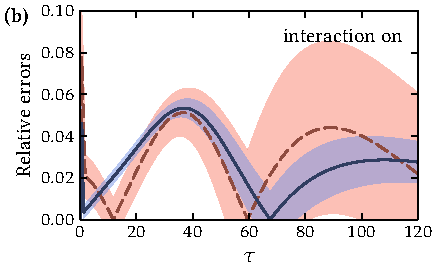
\includegraphics{figures_generated/exact/squeezing_cc_err.pdf}}

    \caption[Sampling and systematic errors in Wigner simulated local squeezing]{
    Relative difference of the Wigner simulated local squeezing and the exact results (solid lines) as compared to the sampling errors in Wigner simulations (dashed lines).
    Plotted are the results for $20,000$ trajectories (red lines) and $200,000$ trajectories (blue lines).
    The plots correspond to \textbf{(a)} the case of no inter-component interaction, and \textbf{(b)} strong inter-component interaction (the interaction coefficients are the same as in~\figref{wigner-bec:mm:squeezing-comparison}).}%endcaption

    \label{fig:wigner-bec:mm:squeezing-error-comparison}
\end{figure}

The expectations above can be expressed in terms of creation and annihilation operators, and calculated either in Wigner representation using \thmref{mm-wigner:mm:moments}, or with the number state expansion using~\eqnref{wigner-bec:mm:exact-a} and~\eqnref{wigner-bec:mm:exact-f}.
The results are plotted in~\figref{wigner-bec:mm:squeezing-comparison}, using a low number of trajectories ($2,000$) to make the sampling error more visible.
The Wigner method shows good agreement with the exact results in the time range of interest; the growing sampling error can be reduced to a desirable extent by using more simulation trajectories.

The relative (normalized on the corresponding exact method results) sampling and systematic errors of the Wigner method are plotted in~\figref{wigner-bec:mm:squeezing-error-comparison}.
The Wigner results show a systematic error in case of turned off interactions at $\tau = 5 \ldots 10$ (\figref{wigner-bec:mm:squeezing-error-comparison},~(a)), which is a sign of the failing truncation approximation.
At other times the difference with the exact results is within the sampling error range.
The large oscillations of the systematic error at the start of the simulation can be explained by accumulating uncertainties in the denominator of~\eqnref{wigner-bec:mm:squeezing}.

Note that while in this particular example the exact method gives more accurate results at comparable or lower computational cost, it becomes unapplicable as soon as one wants to include tunneling and nonlinear losses into the model, while the Wigner method continues to perform with the same effectiveness~\cite{Opanchuk2012a}.
